\documentclass{article}
\usepackage[utf8]{inputenc}


\usepackage{listings}
\usepackage{color}

\usepackage{upgreek}

\usepackage{amsmath}

\usepackage{graphicx}
\graphicspath{ {imgs/} }


\usepackage{xcolor}

\usepackage{xparse}

\NewDocumentCommand{\codeword}{v}{%
\texttt{\textcolor{blue}{#1}}%
}

\lstset{language=C,keywordstyle={\bfseries \color{blue}}}


\hyphenchar\font=-1

\usepackage{enumitem}

\usepackage{listings}

\usepackage{mathtools}
\DeclarePairedDelimiter\ceil{\lceil}{\rceil}
\DeclarePairedDelimiter\floor{\lfloor}{\rfloor}

\usepackage{color}

\usepackage{dsfont}

\usepackage{hyperref}

\usepackage[utf8]{inputenc}

\usepackage{mathtools}

\usepackage{textcomp}

\usepackage[english]{babel}

\usepackage{tikz}

\usepackage{tcolorbox}

\usepackage{amsthm,amssymb}

\setlength{\parindent}{0cm}

\renewcommand\qedsymbol{$\blacksquare$}

\usepackage{fancyhdr}

\pagestyle{fancy}
\fancyhf{}
\fancyhead[LE,RO]{Operating Systems -- Summer 2018}
\fancyhead[RE,LO]{Joshua Concon}
\fancyfoot[CE,CO]{\leftmark}
\fancyfoot[LE,RO]{\thepage}


\title{CSCC69 Lecture Notes}
\author{Joshua Concon}
\date{Summer 2018}

\begin{document}

\maketitle

Textbook: Andrew Tannenbaum: Modern Operating Systems. Prentice Hall (2001 or 2007).

\tableofcontents

\pagebreak

\section{Tuesday, May 8, 2018}

\subsection{What is an operating system?}

To turn "ugly" hardware into "beautiful" abstractions, which essentially means that it makes it easier to use and code on a computer, rather than just using machine code. An operating system also servers as a resource manager and a control program, in the sense that it allocates resources and prevents errors and improper use of the computer.

\paragraph{User Mode} This mode gets requests from applications and the UI and hands it off to the Kernel

\paragraph{Kernel} Processes requests, manages order of requests and implements the requests.

We can imagine the applications running on an OS that connects the running software to the hardware.

\subsection{Storage Hierarchy}

The CPU has cache, which is the smallest and fastest memory in the computer due to it's proximity to the CPU. From there, memory gets larger, slower, cheaper, and further away from the CPU (Think, L2, then L2/L3, then RAM, then HDD,...).

\subsection{Storage Structure}

Main memory (DRAM) stores programs and data during program execution. DRAM cannot store these permanently because it is too small and it is a volatile storage device. Forms a large array of bytes of memory, each with its own addresses. We say that main memory is byte-addressable.

\subsection{Caching}

When the processor accesses info at some level of the storage hierarchy, that info may be copied to a cache memory closer to the processor, on a temporary basis. Since caches have limited sizes, cache management is an important design problem.

\subsection{Concurrency}

Every modern computer is a multiprocessor, so the CPU and device controllers can execute different things, concurrently. A memory controller synchronizes access to a shared memory. \textbf{Interrupts} allow device controllers to signal the CPU that some event has occurred, they are also used to signal errors or requests for OS service from a user program (a \textbf{system call}). These types of interrupts are called \textbf{traps} or \textbf{exceptions}.

Note that an operating system is an event-driven program

\subsection{C Programming and Memory}

A variable in a C program is a symbolic name for a data item, stored in memory. The type of the variable indicates how much \textbf{storage} (how many bytes) it needs. Type also determines \textbf{alignment} requirements. The \textbf{address} of the variable is an index into the big array of memory words where the data item is stored. The \textbf{value} of the variable is the actual contents of memory at that location. A \textbf{pointer} type variable is just a data item whose contents are a memory location (usually the address of another var).

The \textbf{char} data type is 1 byte in size, the \textbf{int} data type is 1 word in size (32 bits for most current architectures), and occupies 4 bytes, should be word-aligned. Pointer types are also 1 word in size.

We'll need to know pointers and the size of types for this course.

\subsection{The Process Concept}

A \textbf{process} can be thought of a program in execution, an instance of a running program. It contains all data of the program, and has a \textbf{PCB (Process Control Block)} and is named by it's \textbf{process ID (PID)}. The PCB contains all of the data of the process, a \textbf{Text} of all the code of the program, a \textbf{Stack} that keeps track of variables and function calls, and a \textbf{Heap} that stores all dynamic memory allocation.

If the stack gets too big and uses more that the space it has, that is called a \textbf{stack overflow}

\subsection{Process Data Structures}

At any time, there are many processes in the system, each in its own PCB. The PCB is also where the OS keeps all of a process' hardware execution state when the process is not running. This state is everything that is needed to restore the hardware to the same configuration it was in when the process was switched out of the hardware.

\subsection{Process Control Block}

It also includes
\paragraph{Process state} (ready, running, blocked,...)
\paragraph{Program counter} which is the address of the next instruction
\paragraph{CPU Registers} their state must be saved at an interrupt
\paragraph{CPU scheduling information} Process priority
\paragraph{Memory Management Info} Page tables
\paragraph{I\slash O status information} list of open files


\subsection{Process state and state changes}

The OS manages processes by keeping tracking of their state. Different events cause changes to a process state, which the OS must record\slash implement.

We need this because one process can't use the CPU forever, we need to switch processes (called Context Switching). So we time-out the process and we save the memory to the PCB for that process when it's time to switch.

Blocked processes can't go to the running state right away, it must wait in the ready state.

\subsection{State Queues}

This is the ready queue.

The OS maintains a collection of queues  that represent the state of all processes in the system. Typically, the OS has one queue for each state, each PCB is queued on a state queue according to its current state. As a process changes state, its PCB is unlinked from one queue and linked to another.

\subsection{PCBs and State Queues}

PCBs are data structures dynamically allocated in OS memory. When a process is created, the OS allocates a PCB for it, initializes, and places it on the Ready queue. As the process computes, its PCB moves from one queue to another. When the process terminates, its PCB is de-allocated.

\subsection{Context Switch}

\paragraph{Context Switch} switch the CPU to another process, saving the state of the old process and loading the saved state for the new process.

Context switch time is pure overhead, so some systems offer specific hardware support. It is also an expensive operation, so many context switches will take a long time, and it is also a performance bottleneck, so new structures are being used to avoid it.

\subsection{Operations on Processes}

Processes execute concurrently and must be created and deleted dynamically.

\subsubsection{Process Creation}

Who can create processes? Users, system initialization, a running process, and batch jobs can create processes.

\subsubsection{Process Termination}

Who can kill processes? when a processes finishes executing, when a parent terminates a child, a user can kill a process, and when an error occurs.

\subsection{Process Creation}

When a process is created by another process, parent is the creator, child is the created. We can use the PPID to differentiate the processes.

In some systems, resources and privileges are inherited from parents to their children. We do this to do concurrency, different processes working on different things.

Parents can either do jobs concurrently with their children, or waits for them.

\subsubsection{Unix}

In Unix, processes are created using fork. fork creates a new address space for the process, and copies the PCB of the parent, and duplicates it with a different PPID. Fork returns twice, returns the child's PID to the parent, 0 to the child, so we can use and if statement to make these two processes do different things.

After this, either the parent or the child could go first, there is no default priority.

Note: a fork duplicating the address space of the original process, so forks are a potentially expensive process.

\subsubsection{Why fork?}

Very useful when the child is cooperating with the parent or when the child relies on the parent's data to accomplish its task. Also easier to do multiple requests at the same time. For example, this would be useful for a websever in handling multiple client requests concurrently.

\subsubsection{Unix Shells}

A shell is a process that gets new commands and executes them. To implement one, receive a command, fork, and the parent waits for the child while the child executes the command.

\subsection{Example: Concurrent Web Server}

If the Text and Data of a PCB are the same, a fork may not be worth the duplication. How can we improve this?

We can improve this by having multiple program counters, split stack resources.

\subsection{Parallel Programming}

Why don't we put them together and make threads? Have threads in a process. These are all on the same PCB and have separate stacks, so it's still a process, but multiple program counters.

Note that every process has at least one thread.

Now we need synchronization, since they all use the same Heap. This means that cost of creating threads is large as well, just like having multiple processes. There is always a tradeoff.

\subsection{Example: Concurrent Servers}

Now with threads, you do a thread\_fork by passing in a request function and all the other arguments for it.

\subsection{Rethinking Processes}

What is similar in these cooperating processes? They all share the same code and data (address space), privileges, and resources (files, sockets, etc.)

What don't they share? Each of them has their own execution state.

\textbf{Key Idea}: Why don't we separate the concept of a process from it execution state?

Execution state is also called a \textbf{thread of control} or \textbf{thread}

\subsection{Threads}

The thread defines a sequential execution stream within a process, while a process defines the address space and general process attributes (everything but thread of execution)

Processes are the containers in which threads execute. Processes become static, and threads are the dynamic entities.

Consider our example with a forking web server, using fork to create new processes to handle requests is overkill for such a simple task, using threads would be more efficient.

\subsection{Thread Interface}

Pthread API will create a new thread for you, can specify priority as well.

\subsection{Thread Scheduling}

The thread scheduler determines when a thread runs, also uses a queue to keep track of what threads are doing. It's just like the OS and processes, but it's implemented at user-level in a library.

How do you implement wait queues? How to wake up a thread?

\subsection{Threads Summary}

The operating system is a large multithreaded program, with each process executing as a thread within the OS.

Multithreading is also very useful for applications. Efficient multithreading requires fast primitives.

\subsection{Cooperating Processes}

Threads are in the same process, so they can communicate through the shared memory (Heap), but processes don't have that space predefined, so we need more support for them. We can use message passing or shared memory. In general, we have independent processes that don't depend on other processes, and dependent processes that are the opposite.

A process is \textbf{independent} if it cannot affect or be affected by the other processes executing in the system.

No data sharing implies that a process is independent. A process is \textbf{cooperating} if it is not independent.

\subsection{Interprocess Communication}

Cooperating processes need to exchange information, using either shared memory or message passing.

\newpage

\section{Tuesday, May 15, 2018}

\subsection{Bootstrapping}

Bootstrapping is the process of bringing up the operating system when you turn on the machine.

The first program that is loaded is the operating system when you turn on your computer, so when the system is off, the operating system is just a program or code that needs to be run.

\paragraph{BIOS} This is the Basic Input Output System, it's job is to just initialize the system, so making sure the hardware is connected and make sure their functioning correctly, scans buses to detect attached decides, determines the boot devices (can access BIOS to change order in which it checks devices, note that people needed to install the operating system separately and had to configure with the BIOS more). This program then reads the first sector of the boot deivce and executes it (this is the bootloader program), then the bootloader reads a partition table, finds the active partition, reads the second boatloader, and then the second bootloader reads the OS into memory and executes it.

\subsection{Operating System Startup}

The Machine starts in system mode, so kernel code can be executed kernel code can be execute immediately.

Then it creates its internal datastructures, creates the first process, switch mode to allow user input and starts running the first process. Then waits for user input, as an OS is entirely driven by external events.

\subsection{Memory Layout}

Note that the OS has its own PCB. This is because the OS itself is a process.

\subsection{From Program to Process}

Consider a program that reboots your computer. We can compile it into an object file and then to create an executable. But that does not mean it can be executed, as it might not have permissions to run.

Note all these files are on the file disk.

\subsection{Unix Shells}

Lets revisit this, a process that waits for commands, and when it recieves one, forks and the child executes the command and the parents continues to wait.

To do this, we use

\begin{lstlisting}
  int exec(char *prog, char *argv[])
\end{lstlisting}

When exec is executed, exec() stops the current process, loads the program "prog" into the process' address space, initializes hardware context and arguments for the new prgram, and places the PCB onto the ready queue

\subsection{Requesting OS Services}

Operating System and user programs are isolated from each other, but the OS provides service to user programs, so how do they commmunicate?

Any communication between the user and the kernel, is a system call, which are all handled by the OS.

\subsection{Boundary Crossings}

Here are some examples of getting to the kernel mode from the user mode:
\begin{itemize}
  \item Boot time (not really a crossing, starts in the kernel)
  \item Explicit system call -- request for service by application
  \item Hardware interrupt
  \item Software trap or exception
  \item Hardware has table of "Interrupt service routines"
\end{itemize}

And for Vice Versa, we have
\begin{itemize}
  \item Jumping to the next application instruction
\end{itemize}

\subsection{System Calls for Process Management}

\paragraph{fork} Creates a child process identical to the parent
\paragraph{waitpid} Waits for a child process to terminate
\paragraph{execve} Replace a process' core image
\paragraph{exit} Terminate process execution and return status

\subsection{System Calls for File Manamgement}

\begin{itemize}
  \item opening and closing files
  \item reading from and writing to a buffer
  \item moving a file pointer with lseek
  \item getting a file's status information with stat
\end{itemize}

\subsection{Systems Call Example}

\begin{lstlisting}
  Read(fd, buffer, nbytes)
\end{lstlisting}

\begin{enumerate}
  \item First we push nbytes to the buffer
  \item we push the file path name
  \item put the code for read in the register
  \item we do a trap to the kernel to do a system call
  \item (Switched to kernel space) we find the code for the read function
  \item it searches for it in a hash table
  \item then passes it to a system call handler, which executes the code
  \item returns to the caller back in the user space
\end{enumerate}

\subsection{System Call Interface}

The system call interface is a C library where the C library functions pass arguments to the OS with a system call identifier. The function also executes a special instruction to trap the system mode. The syscall handler figures out which system call is needed and calls a routine for that operation.

This enforcement of separation between the userspace and kernel is for hardware support.


\subsection{System Call Operation}

There is a fixed number of arguements that can be passed in registers. Often the address of a user buffer containing data (e.g., for \codeword{write()}). The result of the system call is returned in the register

\subsection{Introduction to Synchronization}

\subsubsection{Motivating Example}

Suppose we write functions to handle withdrawals and deposits to a bank account.

The idea is that we create separate threads for each action, which may run at the bank's central server.

But suppose you share this account with someone and the balance is \$1000, you each go to separate ATM machines, you withdraw \$100 and your friend deposites \$100 at the exact same time. But if your process finishes last, you'll end up with \$900, and if their process finishes last, you'll end up with \$1100.

We need synchronization for these processes.

\subsubsection{Interlevced Schedules}

The problems is that the execution of the two processes can be interleaved. One resulting in you ending up with more money and one with you ending up with less money.

\subsubsection{What went wrong}

Two concurrent threads manipulated a shared resource without any synchronization. The outcome depends on the order in which accesses take place, this is called a \textbf{race condition}. We need synchronization to ensure that only one thread at a time can manipulate the shared resource.

\subsubsection{Revisiting the Example}

$T_1, T_2$ share $X$, $T_1$ increments $X$ by 1 and $T_2$ decrements $X$ by 1. This is the same problem, since at the machine level, we load it from a register, performing the increment or decrement, and then store it back. This is basically the same bank account problem.

\subsubsection{Mutal Exclusion}

To solve this problem, we need to define it.

Given a set of $n$ threads $T_0, ..., T_n$, a set of resources shared between threads, and a segment of code which accesses the shared resources, called the \textbf{critical section (CS)}.

We want to ensure that only one thread at a time can execute in the critical section, and all other threads are forced to wait on entry, when a thread leaves the CS, another can enter.

\subsubsection{What program data is shared between threads?}

Local variables are not shared, since each thread has its own stack and local vars are allocated on that.

Global variables and static objects are shared, they are stored in the static data segment, accessible by any thread.

Dynamic objects and other heap objects are shared as well.

\subsubsection{The Critical Section Problem}

To solve this problem, we need to design a protocol that threads can use to cooperate (code for entering the CS code and code for exiting the CS code).

Each thread must request permission to enter its CS in its \textbf{entry} section, the CS may be followed by an \textbf{exit} section, the remaining code is the \textbf{remainder} section.

\subsubsection{Critical Section Requirements}

We need to design a protocol that threads can use to cooperate.
\begin{enumerate}
  \item Mutual Exclusion, If one thread is in the CS then no other is.
  \item Progress, If no thread is in the CS and some thread want to enter CS, it should be able to enter in definite time.
  \item Bounded waiting (no starvation), If some thread $T$ is waiting on the CS, then there is a limit on the number of times other thread can enter the CS before this thread is granted access.
  \item Performace, The overhead of entering and exiting the CS must be small with respect to the work being done on it. This is the most important.
\end{enumerate}

\subsubsection{Some Assumptions and Notation}

Assume no special hardware instructions, no restrictions on the number of processors.

Assume that basic machine language instructures (like LOAD, STORE, etc.) are atomic, cannot be interrupted.

If there are only two threads, we number them $T_0$ and $T_1$

\subsubsection{2-Thread Solutions: First Attempt}

Let the threads share an integer variable turn that if
\begin{lstlisting}
  turn = i
\end{lstlisting}
then thread $T_i$ is allowed into its CS.

In the code.
\begin{lstlisting}[language=c]
  while (turn != id);
  /* this means to keep checking until it is
  your id, when it is, continue.*/
  turn = 1 - id
\end{lstlisting}

What is the problem with this? It's bad because there is no prioritizing in it. The example given is that if $T_0$ is hungry and $T_1$ is not hungry and it's $T_1$ turn to access the critical section (which is food in this metaphor), then $T_0$ has to wait for $T_1$ to get hungry and eat from the CS.

\subsubsection{2-Thread Solutions: Second Attempt}

First attempt does not have enough about state of each process, it only remembers which process is allowed to enter its CS.

So in the second implementation, we use 2 booleans, if one boolean is true, the other threads will not enter the CS, and will only enter when the other person's boolean is false.

The problems with this is when both booleans are false, then nothing is done, and when context switch happens before the flag can be declared. This method is not atomic (mutual exclusion is not guaranteed). We can't fix this by changing the order of testing and setting flag variables, this can lead to a deadlock.

\subsubsection{2-Thread Solutions: Third Attempt}

Combine two key ideas of first two attempts.

The threads share the variables turn and flag, where the flag is an array like before. Check for both the turn variable and the flag boolean to be correct in the while loop.

This means a thread is checking that it wants to enter the CS, and that the other thread is not in the CS.

This is \textbf{Peterson's Solution}.


\subsubsection{Synchronization Hardware}

To build these higher-level abstractions, it is useful to have some help from the hardware.

\subsubsection{Atomic Instructions: Test-and-Set Lock (TSL)}

No interruptions, but this lock can have multiple instructions.

This uses a lock variable, which is 0 means that nobody is using the lock, and 1 means the lock is in use. Hardware executes this automatically

\begin{lstlisting}
  boolean test_and_set(boolean *lock){
    boolean old = *lock;
    *lock = True;
    return old;
  }
\end{lstlisting}

The semantics of this are:
\begin{itemize}
  \item Record the old value of the variable
  \item Set the variable to some non-zero value
  \item Return the old value
\end{itemize}

This code returns True when in use and False when it is not in use, but then the caller "acquires" the lock.

So in the implementation, an \codeword{acquire()} function checks if the lock is available, and if it returns false, it has been acquired, and a \codeword{release()} function sets the lock back.

This is a \textbf{spinlock}, uses \textbf{busy waiting}, so the thread continually executes the while loop in the acquire function, this consumes CPU cycles, so it is wasting CPU cycles.

\newpage

\section{Tuesday, May 22, 2018}

\subsection{Producer and Consumer}

This is about two processes sharing a limited buffer, the producer puts info into the buffer and the consumer takes info out. It's bad if the consumer consumes nothing and the producer overfilling the buffer so how do we solve this. Our solution is to sleep when we can't perform our action and wake up when we can, so the producer will sleep when the buffer is full and the consumer will sleep when the buffer is empty, and they will both be wake otherwise.

If the buffer has a max size of $N$, we wake up the producer when it is of size $N-1$ because they sleep when it reaches $N$, and the consumder sleeps when it reaches 0, and wakes up when the size is $1$.

This is a more relaxed approach, as opposed to always checking.

\subsection{Semaphores}

These are abstract data types that provide synchronization. They include:
\begin{itemize}
  \item An integer variable, accessed only through 2 atomic operations.
  \item The atomic operation \textbf{wait} that decrements the variable and block until semaphore is free
  \item{The atomic operation \textbf{signal} that decrements the variable and unblocks a waiting thread if there is any}
  \item a queue of waiting threads
\end{itemize}

\subsubsection{Types of Semaphores}

\begin{itemize}
  \item Binary or Mutex
  \begin{itemize}
    \item Represents a single access to a resource
    \item guarantees mutual exclusion to a critical section
  \end{itemize}
  \item Counting Semaphores
  \begin{itemize}
    \item Represents a resource with many units available, or a resource allowing certain kinds of unsynchronized concurrent access.
    \item Multiple threads can pass the semaphore
    \item max number of threads is determined by semaphore's initial value, $count$
  \end{itemize}
\end{itemize}

This is similar to locks, but semantics are different.

We must ensure that two threads cannot execute wait and signal at the same time though. This is another critical section problem, which we can solve with using lower-level primitives, Uniprocessors to disable interrupts and Multiprocessors, using hardware instructions.

\subsection{The reader, writer problem}

Consider the following
\begin{itemize}
  \item An object is shared amount several threads
  \item Some only read the object, others only write it, we allow multiple concurrent readers, but only one writer. How can we implement this with semaphores.
\end{itemize}

This is a problem because the writer conflicts with all of the readers. Another critical section.

To solve this, we need 3 variables
\\
\\
One binary semaphore, that is exclusive to reading or writing. This means that either the one writer is writing or $\geq 1$ readers are reading. Which thread in the group of readers is in charge of getting and returning the token? Who will return the token? The last one. "The last to leave the room turns off the light."
\\
\\
We also need an integer that keeps track of the number of threads reading the object, this is how we detect when a reader is the first or last of a group.
\\
\\
Finally, we need another binary semaphore for control access to readcount.
\\
\\
For implementation, the writer just needs to wait for its global token, once it gets it, writes, and puts the global token back. For the reader, they wait  for the read token, then they wait for the global token, once they get it, increment the read count, and then return the token, and when they leave, if read count is 1 (the last reader), they put the global token back.
\\
\\
What if the first reader arrives while the writer is active? What happens? Then they wait for the global token. Then the second reader will wait for the read count token in this scenario if there was a second reader.

\subsection{Monitors}

It's to easy to make mistakes with counting semaphores. For example, we could accidentally wait for the global token twice or signal twice.

Monitors are an abstract data type with the restriction that only one process at a time can be active within the monitor. This protects local data accessed only by the monitor's procedures, and a process enters the monitor by invoking 1 of its procedures, and other processes that attempt to enter monitor are blocked.\\
\\
But what if a process in the monitor may need to wait for something to happen? Then that process has to leave and to let another process use the monitor. This provides a special type of variable called a \textbf{condition}. The operations on a condition variable are \textbf{wait}, to suspend the invoking process, and \textbf{signal}, to resume exactly one suspended process.

But what happens if there is one process $P$ in the monitor and it signals the second process $Q$, waiting in a condition.
\begin{itemize}
  \item $P$ is already in the monitor, so it does not neat to block.
  \item $Q$ becomes unlocked by the signal, and want to resume exection in the monitor.
  \item But both cannot be simultaneously active in the monitor.
\end{itemize}

There are 3 solutions
\begin{itemize}
  \item Hoare Monitors
  \begin{itemize}
    \item \codeword{signal()} immediately switches from the caller to a waiting thread
    \item Need another queue for the signaler, if signaler was not done using the monitor
  \end{itemize}
  \item Brinch Hansen Monitors
  \begin{itemize}
    \item Signaler must exit monitor immediately, so \codeword{signal()} is always the last statement in the monitor procedure
  \end{itemize}
  \item Mesa Monitors
  \begin{itemize}
    \item \codeword{signal()} places a waiter on the ready queue, but signaler continues inside monitor
  \end{itemize}
\end{itemize}

So how can we implement the readers / writers problem with Monitors?

\subsubsection{Bounded Buffer Problem}

Consider Producers that want to add to the buffer and Consumers that want to remove from the buffer. So we want to use a Monitor for the buffer, so that only one operation is done at a time, there needs to be one lock, and two conditions, one to make consumers wait, and one to make producers wait.

In terms of implementation, we're going to have an index for where the producers can insert and an index for where consumers can remove. The buffer will be a circular buffer, so adding to the indexes will also be the $mod$ of the largest index of the buffer.

If a consumer $C$ enters the monitor and the buffer is empty, the consumer waits on a condition for a producer to put stuff in the buffer and signals the $C$ or another consumer on the enter queue can enter the monitor.

\subsection{Process Scheduling}

So we have scheduling at different levels of the Operating Systems.

For CPUs, only one process can run at a time on a CPU, the Scheduler decides which process to run and the Goal of CPU scheduling is to give the illusion that processes are running concurrently and maximizing CPU utilization.

\subsubsection{What happens on a dispatch \slash context switch?}

When switching the CPU to another process
\begin{enumerate}
  \item The current process using the CPU is having it's state saved (unless it's going to be exiting)
  \item The next process is selected from thr ready queue
  \item Then the state of the next process is restored, such as registers.
  \item Kernel mode switches to user mode
  \item The PC is set to the next instruction in the new process
\end{enumerate}

\subsubsection{Process Life Cycle}

Processes repeatedly alternate between computation and I\slash O.
\begin{itemize}
  \item This is called CPU burts and I\slash O bursts.
  \item The last CPU burst ends with a call to terminate the process.
\end{itemize}

\paragraph{I\slash O - Bound Processes} These processes have short CPU bursts and frequent (long) I\slash O bursts
\paragraph{CPU - Bound Processes} These processes long CPU burts and infrequent I\slash O bursts

During I\slash O bursts, CPU is not needed, this is an opportunity to execute another process.

\subsubsection{What is processor scheduling?}

The allocation of processors to processes over time. This is the key to \textbf{multiprogramming}. We want to increase CPU utilization and job throughput by overlapping I\slash O and computation.\\
\\
We also have to consider \textbf{Policies} in multiprogramming. For example:
\begin{itemize}
  \item Given more than one runnable process, how do we choose which to run next?
  \item When do we make this decision?
\end{itemize}

We schedule these process changes:
\begin{itemize}
  \item When the running process blocks or exists, such as Operating System Calls (I \slash O)
  \item At fixed intervals, such as clock interrupts
  \item When a process enters the Ready state, such as I \slash O interrupts, signals, and process creation.
\end{itemize}

\subsubsection{Scheduling Goals}

For all systems:
\begin{itemize}
  \item we want \textbf{Fairness}, in that each process recieves a fair share of the CPU
  \item Avoiding \textbf{starvation} (a process waiting too long)
  \item \textbf{Policy Enforcement} -- Usage policies should be met
  \item Balance -- That all parts of the system should be busy
\end{itemize}.

For batch systems
\begin{itemize}
  \item Throughput -- we want to maximize the jobs completed per hour
  \item Turn around time -- We wanna minimize the time between submission and completion
  \item CPU Utilization -- keep the CPU busy all the time.
\end{itemize}

For interactive systems
\begin{itemize}
  \item we want to minimize response time, time between recieving the request and starting to produce output
  \item Proportionality -- "simple" tasks complete quickly while more "complicated" ones take longer
\end{itemize}

For real-time systems
\begin{itemize}
  \item Deadlines must be met
  \item Must be predictable
\end{itemize}

Note that goals sometimes conflict with each other

\subsubsection{Types of Scheduling}

\paragraph{Non-preemptive scheduling} One the CPU has been allocated to a process, it keeps the CPU until it terminates. This is suitable for batch scheduling.

\paragraph{Preemptive Scheduling} CPU can be taken from a running process and allocated to another. Needed in interactive or real-time systems.

\newpage

\section{Tuesday, May 29, 2018}

\subsection{Problem: Dining Philosophers}

A philosopher needs two forks to eat, 5 philosophers with 5 meals sharing 5 forks.
\\
\\
One idea of a solution is that if a philosopher gets hungry, grab a left fork and a right fork. But if they all get hungry at the same time, they will all have one fork and can't eat. So we're looking for a better solution.
\\
\\
In the previous non-solution, we only had 2 states, "eating" and "thinking", but in the following solution, we'll have 3 states, "eating", "hungry", and "thinking". One semphore for each philosopher. The Philosopher will think, then call a \codeword{take_forks()} function, eat, and then calls a \codeword{put_forks()} function. We also need a mutex for entering and exiting the critical section of eating.\\
\\
What does the \codeword{take_forks()} function do? It enter's the critical region with a mutex, since the philosopher and the two philosophers next to that person can change their state. It then calls another function called \codeword{test()}, that changes the state to eating if the philosophers next to the one we're currently refering to are not eating, and then exits the critical region. Changing the state to hungry is a critical state since 3 people can change one person's state for all philosophers. The semaphores are used since if \codeword{test()} fails since there are not enough forks to eat, then that philosopher will be blocked until a fork is returned, since their semphore cannot be decremented.\\
\\
After a philosopher finishes eating, he will put down his forks, in teh sense that he will check if the two people sitting next two him want to eat and have access to their other fork.

\subsection{Scheduling Algorithms}
\subsubsection{FCFS}
"First come, first serve", all you need is a queue, so it's very easy to implement. However, has no prioritization.\\
\\
It's problem whoever that it's average waiting time is often quite long and causes the:

\paragraph{Convoy effect} All other processes wait for the one big process to release the CPU


\subsubsection{SJF}

"Shortest Job First", this is better, but we need to know the processing time in advance. It also does not take into account fairness and starvation.

\subsubsection{Round Robin}
Designed for time-sharing system, is a pre-emptive algorithm. Here the ready queue is circular, each process is allowed to run for time quantum $q$ before being preempted and put back on queue. This is good, but the choice of quantum is critical, the bigger it is, the closer the algorithm is to FCFS, and the smaller it is, the more it becomes like processor sharing, which is inefficient.\\
\\
However, there is also no prioritization in this solution as well. If we want to enforce prioritization, it would be tricky, like multiple queues. This may cause starvation or priority inversion, as low priority tasks may never run and low priority tasks may prevent high priority tasks from making progress by holding a resource.

\subsubsection{Mars Rover Pathfinder Bug Example}

The Mars Rover was not making progress being it kept doing context switches, and left all of its work in the shared memory before the context switch. This is priority inversion, as a high priority tasks now has a smaller amount of space on the shared memory to work with

\subsection{What do real systems do?}

Real systems us a combination of Multilevel queue scheduling, like Round Robin with priorities and Feedback Scheduling, which is adjusting the quantum accordingly by feedback of real usage.

\subsubsection{Multi-Level Queue Scheduling}

There is going to be two scheduling policies here, the first decides which queue to serve (e.g. based on queue priorities), and second decides which job within a queue to choose.
\\
\\
So in an implementation, a quantum of a lower priority queue would be longer than a quantum of a higher priority queue. So if a highest priority task finishes during quantum, that is a good result, but if not, the task is bumped into second highest priority. This means that the shortest high priority jobs get done first, and that the processes are ordered by how long they take, so we now know if they are short or long jobs.

\subsubsection{Feedback Scheduling}

We want to give priority to shorter jobs, IO bound jobs, and to interactive jobs, but we don't know beforehand whether a job is short or long and whether it's IO bound or CPU bound.\\
\\
We can adjust criteria for choosing a particular process based on past history, such as Multi-Level Queues, can prefer processes that do not use full quantum, can change priority of porcesses based on age, can change priority of processes based on CPU consumed so far, can boost priority following a user-input event.



\subsubsection{Timesharing in Linux 2.8}

Linux always runs the task in the active array with the highest priority, if there are other processes with the same priority, do round robin between then and switch after granularity time units.\\
\\
If timeslice expires, move to the expired array. This way, tasks are being re arranged and prevents starvation.\\
\\
But how do we determine priority of a process?\\
\\
Some processes are more important than others, so static priorities are assigned to processes, and bonuses are added or subtracted depending on if it's an interactive and \slash or IO bound processes, which can be identified by sleep average (time process has the CPU does not do anything, which is time process is sleeping vs its CPU time.)
\\
\\
How do we determine timeslive and granularity?
\\
\\
Timeslice depends on static priority, which for example, can be anywhere from 5 to 800 milliseconds and Granularity depends on a dynamic priority

\newpage

\section{Tuesday, June 5, 2018}

\subsection{Memory Management}

Every active process needs memory and CPU scheduling allows processes to share the processor. So we should figure out how to share main memory as well.\\
\\
So for this section, in terms of Memory Management, we want to support enough active processes to keep the CPU busy, Use memory efficiently in that we minimize wasted memory, and keep memory management overhead small.

\subsubsection{Requirements}

\paragraph{Relocation} When allocating memory for a process, we won't know what physical memory will be available when their programs run and the scheduler may swap processes in and out of memory, so we need to be able to bring back a process into a different region of memory. This implies that we will need some type of address translation.

\paragraph{Logical Organization} The machine accesses memory addresses as a one dimensional array of btyes, and programmers organize code into modules, so we need to map these two views together

\paragraph{Protection} A process' memory should be protected from unwanted access by other processes, both intentional and accidental, this requires hardware support.

\paragraph{Sharing} In some instances, processes need to be able to access the same memory locations, so we need ways to specify and control what kind of sharing is allowed.

\paragraph{Physical Organization} Memory and Disk form a two-level hierarchy, flow of information between levels must be managed. This is because the CPU can only access data in registers or in memory, not the disk.

\subsubsection{Meeting the Requirements}

Modern systems use \textbf{virtual memory}, which is a complicated technique requiring hardware and software support. We'll build up to virtual memory by looking at some simpler schemes first, such as Fixed and Dynamic partitioning, Paging and Segmentation.

\subsubsection{Address Binding}

Programs must be in memory to execute, so a program binary is \textbf{loaded} into a process, so we need to allocate memory for the instructions and the data.\\
\\
And these addresses in programs must be translated to real addresses since Programmers use \textbf{symbolic memory addresses} (i.e. variable names) to refer to memory locations and the CPU fetches from, and stores to \textbf{real memory addresses}

\subsubsection{When are addresses bound?}

\paragraph{Compile Time?} This is called \textbf{absolute code} since binary contains real addresses. The disadvantage of this is that we must know what memory process will use during compilation and no relocation is possible.

\paragraph{Load Time?} Compiler translates (binds) symbolic addresses to \textbf{logical, relocatable addresses} within a compilation unit (source file). So a linker takes a collection of object files and translates these addresses to logical, absolute addresses within the executable, which resolves references to symbols defined in other files or modules. The loader translates logical, absolute addresses to physical addresses when program is loaded into memory.\\
\\
Disadvantages are that programs can be loaded to different addresses when they start, but cannot be relocated later.

\paragraph{Execution Time?} The executable object file, \codeword{a.out}, contains addresses for the entire program, this is good for translation to physical addresses as relocation is easier, but this requires special hardware.

\subsubsection{Address Translation: Logical and physical addresses}

The source code uses \textbf{symbolic addresses} (variable names), and is compiled to a program binary that uses \textbf{logical addresses} (relative to start of stack frame), the program binary is then loaded and executed as a process, where the logical addreses need to be translated to physical addresses.\\
\\
For now, we'll assume that the entire address space of process must be in the main memory and a process uses a contiguous chunk of main memory.

\subsubsection{Fixed Partitioning}

This is dividing memory into regions with fixed boundaries, which can be equal or unequal sizes. A single processes can be loaded into each remaining partition. However, the disadvantages of this is that Memory is wasted if any single process is smaller than a partition (this is called \textbf{internal fragmentation}), and that Programmers must deal with programs that are larger than a partition, this is called \textbf{overlays}.
\\
\\
Note that the number of partitions determines the number of active processes and if all paritions are occupied by waiting processes, some processes need to swap out.\\
\\
Equal-sized paritions means that processes can be loaded into any available partition and unequal-sized paritions need a queue for each partition and for each process, we'll add it to the queue of the smallest partition in which it will fit or have a single queue and assign a process to the smallest available parition.

\subsubsection{Dynamic Partitioning}

Paritions will vary in length and number over time, so when a process is brought into memory, a partition of the right size is created to hold it.
\\
\\
Disadvantages of this is that as some processes come and go, "holes" are created, and some blocks may be too small for any process, this is called \textbf{external fragmentation}.\\
\\
The Operating System may also move processes around to create larger chunks of free space, this is called \textbf{compaction} and requires processes to be relocatable.

\subsubsection{Heap Manamgement}

How is dynamic memory management implemented (\codeword{malloc() \slash free()})? This is done with a dynamic partitioning system to maintain a contiguous range of logical addresses, and allow allocating and deallocating of dynamic memory.

\subsubsection{Tracking Memory Allocation}

We could try using bitmaps where 1 bit represented one allocation unit, and 0 meant free and 1 meant allocated, to track memory allocation. The disadvantages of this is that allocating a $N$-unit chunk takes $O(N)$, which is slow.\\
\\
Another implementation is a linked lists of allocated and free segments, but we would need to store it, Lists need memory too.\\
\\
We should have each block to have a header that records its size and status (used or free) so searching for free blocks is only linear in total number of blocks. We can also store pointers in the free blocks to create a doubly-linked list.\\
\\
Freeing Blocks would result in surrounding free blocks to merge, this will be easier if all blocks end with a footer with size and status info (called a \textbf{boundary tag}).

\subsubsection{Placement Algorithms}

Compaction is time-consuming and not always possible. We can reduce the need for it by being careful about how memory is allocated to processes over time. Given multiple blocks of free memory of sufficient size, how should we choose which one to use.\\
\\
\paragraph{First-fit} choose first block that is large enough; search can start at beginning, or where previous search ended (called next-fit). This is the simplest and often the fastest and most efficient, but it may leave small fragments near start of memory that must be searched repeatedly

\paragraph{Best-fit} choose the block that is closest in size to the request. However, left over fragments tend to be so small that they are so unusable. In practice, similar storage utilization to frist-fit.
\paragraph{Worst-fit} choose the largest block. Not as good as best-fit or first-fit in practice.
\paragraph{Quick-fit} keep multiple free lists for commmon block sizes. This is great for fast allocation, generally harder to coalesce.

\subsubsection{Problems with Partitioning}

With fixed partitioning, \textbf{internal fragmentation} and need for overlays are big problems, so this scheme is too inflexible. With dynamic partitioning, \textbf{external fragmentation} and management of space are major problems. The basic problem is that processes must be allocated to contiguous blocks of physical memory, so its hard to figure out how to size these blocks given that processes are not all the same.\\
\\
We'll look now at paging as a solution

\subsubsection{Paging}

Partition memory into equal, fixed-size chunks. These are called \textbf{page frames} or simply \textbf{frames}. Then divide processes' memory into chunks of the same size, these are called \textbf{pages}.\\
\\
Possible page frame sizes are restricted to powers of 2 to simplify translation.\\
\\
This results in an elimination of external fragmentation, and internal fragmentation is at most, a part of one page per process.

\subsubsection{Address Translation}

Swapping and compaction require a way to change the physical memory addresses a process refers to, so we really need dynamic relocation (aka execution-time binding of addresses). Note that this process refers to relative addresses, hardware translates to physical addresses as instruction is executed.\\
\\
We assume that all memory used by any process is contiguous in these methods. The basic idea for hardware for relocation is that we add relative addresses to process statarting addresses (or base addresses) to form real, or physical, addresses. This is to check that the address generated is within the process's space.\\
\\
2 registers will store the "base" and "limit" of the process. When a process is assigned to a CPU, the "base" register will be loaded with the starting address of the process, and the "limit" register will be loaded with the last address of the process.\\
\\
This is all done in hardware by a Memory Management Unit (MMU).

\subsubsection{Address Translation for Paging}

So now we need more than just the base and limit registers now. Operating systems maintain a \textbf{page table} for each process. This page table records which phyiscal frame holds each page, so
$$\text{virtual address} = \text{page number} + \text{page offset}$$

$$\text{page number} = \text{virtual address} + \text{page size}$$

$$\text{page offset} = \text{virtual address} \% \text{page size}$$

These calculations are really simple if page size is a power of 2.\\
\\
On each memory reference, processor translates page number to frame number and adds offset to generate a phyiscal address. So a "page table base register" is kept to quickly locate the page table for the running process.

\subsubsection{Page Table Entries (PTE)}

Page table entries control mapping. They contain a \textbf{modify bit} that says whether or not a page has been written and is set when a write to a page occurs, a \textbf{reference bit} that says whether a page has been accessed and is set when a read or write to a page occurs, a \textbf{valid bit} says whether the PTE can be used, and is checked on each used of the virtual address. PTEs also contain \textbf{Protection Bits} that specify what operations are allowed on the page (such as read, write, and execute), and the \textbf{Page frame Number (PFN)} determines the physical page it refers to.\\
\\
Note that not all bits are provided by all architectures.

\subsubsection{Page Lookups}

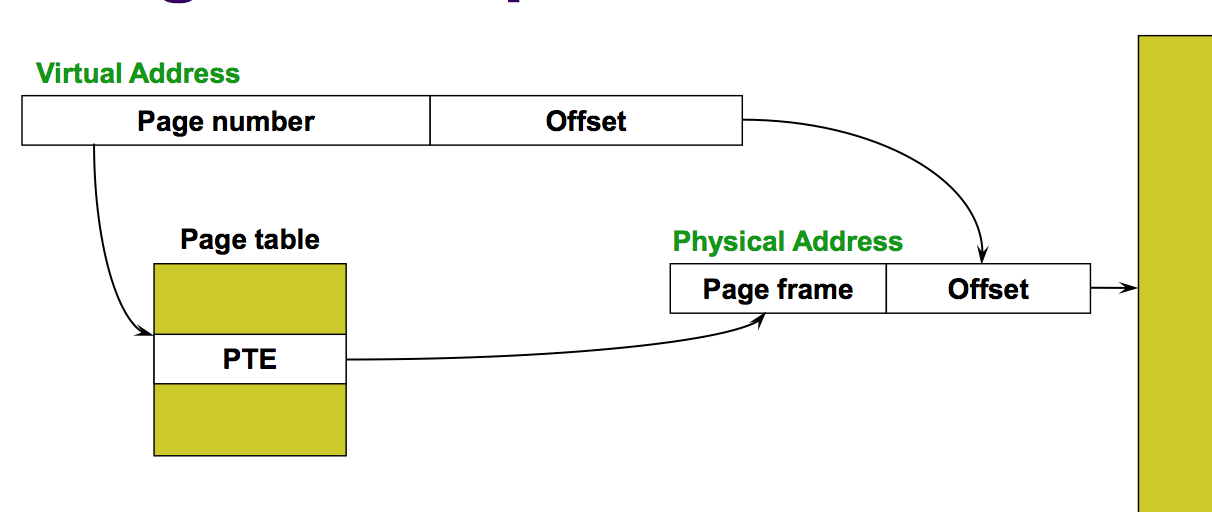
\includegraphics[scale=.50]{pagelookup}

This approach is wrong since it needs 2 references for address lookup, one for the page table and the other for the actual memory. The idea is to use hardware cache of page table entries called a \textbf{Translation Lookaside Buffer (TLB)}, which stores recently used translations.

\subsubsection{Translation Lookaside Buffer}

These translate virtual page numbers into PTEs (not phyiscal addresses), and can be done in a single machine cycle.\\
\\
TBLs are implemented in hardware with Fully associative cache (so that all entries are looked up in parellel, cache tags are virtual page numbers, cache values are PTEs). With the Page table entry and the offset, we can directly calculate the physical address.\\
\\
TLBs are small, only varying from 64-1024 entries, and address translations for most instructions are handled using the TLB (~99\%). If the PTE is found in the TLB, this is called a \textbf{TLB Hit}, and if it isn't and the page table in memory needs to be checked, this is called a \textbf{TLB Miss}.
\\
\\
TLBs are effective because of locality, Processes only use a handful of pages at a time and so we only need to "map" those pages. Hit rates are therefore very important.

\subsubsection{Managing TLBs}

Who places translations into the TLB?\\
\\
(Hardware Solution) The Memory Management Unit knows where page tables are in main memory, and are accessed by the MMU directly as the OS maintains the tables. Tables also have to be in a hardware defined format for the MMU.\\
\\
(Software Solution) The OS places them. The TLB faults to the OS, the OS finds the appropriate PTE, and loads it into the TLB. This however, must be fast, and the CPU ISA has instructions for manipulating the TLB. In this solution, tables can be in any format convenient for the OS.\\
\\
The OS ensures that the TLB and page tables are consistent, so that when it changes the protection bits of a PTE, it needs to invalid that same PTE if it is in the TLB.\\
\\
TLBs are reloaded on a process context switch, and since it's more efficient to just invalidate all the entries instead of selecting specific ones, that is done on a context switch.\\
\\
When the TLB misses and a new PTE has to be loaded, the cached PTE must be evicted. Choosing a PTE to evict is called the \textbf{TLB replacement policy}, and is implemented in hardware, and is often very simple.

\newpage

\section{Tuesday, June 12, 2018}



\newpage

\section{Tuesday, June 19, 2018}

\subsection{Eviction Algorithm}

\subsubsection{Least Recently Used (LRU)}

LRU uses reference information to make a more informed replacement decision. The idea is that we can't predict the future, but we can make a guess based upon past experience. On replacement, we evict the page that has not been used for the longest time in the past, which is Belady's future.\\
\\
To implement this, we need to timestamp every page, and sort them to get the LRU page.
\\
\\
Well, the first problem is that we need to sort every time we evict, and where do we store the timestamp? That's something we have to store for every page. Sorting can also be costly.
\\
\\
We can try keeping pages in a stack, on reference, move a page to the top of the stack, and on eviction, replace page at the bottom, but is also very costly to manipulate stack on every memory reference.\\
\\
We don't implement the exact LRU, but we can use approximations by the PTE reference bit. The basic idea is that initially, all $R$ bits are zero; as processes execute, bits are set to 1 for pages that are used, so we periodically examine the R bits, we do not know order of use, but we know pages that were or were not used.\\
\\
Additionally, we can also have a reference bit algorithm where we keep a counter for each page, and at regular intervals, for each page, we shift $R$ bit into high bit of counter register, shift the other bits to the right, and pages with "larger" counters were used more recently.

\subsubsection{Counting-based replacement}

You can also count the number of uses of a page, here are the uses:
\paragraph{Least-Frequently-Used (LFU)} Replace the page used least often, pages that are heavily used at one time tend to stick around even when not needed anymore. Newly allocated pages haven't had a change to be used much though.

\paragraph{Most-Frequently-Used (MFU)} This algorithm favours new pages.

Neither of them is common, both are poor approximations of OPT.

\subsubsection{Fixed vs. Variable Space}

In a multiprogramming system, we need a way to allocate memory to competing processes. The problem is, how do we determine how much memory to give each process? There are two solutions.

\paragraph{Fixed Space Algorithms} Each process is given a limit of pages it can use, when it reaches the limit, it replaces from its own pages, but some processes may do well with this system while others may suffer.

\paragraph{Variable Space Algorithms} Process' set of pages grows and shrinks dynamically, however, one process can take up all the possible space, and replacement and set size are separate, so replacement is hard.

\subsubsection{Working Set Model}

How do you decide how large the fixed or variable space for a process should be?\\
\\
A Working Set of a process is used to model the dynamic locality of its memory usage. The definition is
$$WS(t,\Delta) = \{ \text{pages $P$ such that $P$ was referenced in the time interval $(t, t-\Delta)$} \}$$
$$t=\text{time}$$
$$\Delta = \text{working set window (measured in page references)}$$

A page is in the working set (WS) only if it was referenced in the last $\Delta$ references.\\
\\
The working set size is the number of pages in the working set, the number of pages referenced in the interval $(t,t-\Delta)$.\\
\\
The working set size changes with program locality. During periods of poor locality, you reference more pages, and within that period of time, the working set size is larger.\\
\\
Intuitively, we want the working set to be the set of pages a process needs in memory to prevent heavy faulting, so each process has a parameter $\Delta$ that determines a working set with few faults.

% Switches slides at this point, I didn't copy everything

\subsection{File Systems}

What do file systems do? They provide a nice abstraction of storage.

\end{document}
